\documentclass[runningheads,twocolumn,envcountsame,envcountsect]{llncs}
\usepackage[T1]{fontenc}
\usepackage{lmodern}
\usepackage{amsmath,amssymb,booktabs,tabularx,array,graphicx}
\usepackage{enumitem,xcolor,tikz,microtype,xurl}
\usepackage{hk261_compact}
\usepackage[hidelinks]{hyperref}
\usetikzlibrary{arrows.meta,positioning,fit,backgrounds,calc}
\definecolor{ink}{gray}{0}
\definecolor{teal}{gray}{.18}
\definecolor{blue}{gray}{.28}
\newcolumntype{P}[1]{>{\raggedright\arraybackslash}p{#1}}
\newcolumntype{Y}{>{\raggedright\arraybackslash}X}
\newcommand{\E}{\mathbb E}
\newcommand{\TV}{\operatorname{TV}}
\newcommand{\Var}{\operatorname{Var}}
\newcommand{\Cov}{\operatorname{Cov}}
\newcommand{\BQ}{GeoI-BQ}
\hypersetup{pdftitle={GeoI-BQ: Bounded Transcript Disclosure for Road-Aware Location Queries},
pdfauthor={Hanh Ngo-Minh; Phan Trong Nhan},
pdfsubject={HK261 template-based compact author-review manuscript}}
\title{GeoI-BQ: Bounded Transcript Disclosure for Road-Aware Location Queries}
\titlerunning{GeoI-BQ: Bounded Transcript Disclosure}
\author{Hanh Ngo-Minh \and Phan Trong Nhan}
\authorrunning{Hanh Ngo-Minh and Phan Trong Nhan}
\institute{}
\newcommand{\paperabstract}{%
\begin{abstract}
Repeated location queries expose a transcript whose privacy cannot be inferred from
isolated noisy points. We present GeoI-BQ, combining a geo-indistinguishable road
reference, private reference reuse and bounded joint query-segment sampling.
A summable allowance schedule limits transcript disclosure without specifying trip
duration. Under explicit support, timing, state and provider assumptions, we derive
an end-to-end likelihood-ratio bound and prior-dependent localization guarantees.
Utility analysis separates planning-score gain from actual service reward and bounds
deviation from a matched public base. A controlled synthetic comparison with three
audited paper adaptations and two controls uses 20 test families and 120 retained
trip-draws. GeoI-BQ achieves 99.595\% session Recall@5 and 0--0.188\% Hit100 across
five localization tasks, using 155 coordinate queries per 600-second session.
The nonadaptive base has slightly higher Recall, and complete static-reference
access limits claims of online necessity. These findings support a conditional
transcript mechanism and reproducible trade-off analysis, rather than deployment
certification or faithful reproduction of the original papers.

\keywords{Trajectory privacy \and Geo-indistinguishability \and
Location-based services \and Adaptive composition \and Point-of-interest retrieval}
\end{abstract}}
\begin{document}
\maketitle
\section{Introduction}\label{sec:intro}
Map services help travellers find routes and nearby places. Repeated trips ending near a hospital could invite inferences about a person's health or routine, even if the traveller is visiting a relative. The distinctiveness of mobility traces makes this concern relevant across repeated queries~\cite{mobilityunique}.

How much does the exchange over an entire trip help the provider distinguish
two possible trajectories? Geo-indistinguishability (Geo-I) gives a starting
point by bounding the likelihood ratio for the same output at two true
locations~\cite{geoi}. Extending that argument to a session requires accounting
even for GPS reads that help the phone decide whether to keep its previous
reference. Predictive privacy mechanisms likewise account for the cost of
fresh observations~\cite{predictive}.

For the traveller, what matters is which points of interest (POIs) appear in
the answer. Several query locations can retrieve enough candidates for the
phone to rank them using the private request~\cite{ev}. We therefore compare
the answer the user receives with the full-catalogue answer to the same request
at the true GPS position. This comparison accommodates a single replacement
coordinate, a set of real and dummy locations, or a stream with extra fake
queries. Offline trajectory releases serve a different downstream
task~\cite{transprotect,semantic,fake,sok}.

We distinguish ten scenarios by what the observer tries to infer and which
part of the exchange (the transcript) is available.

\smallskip\noindent\textbf{Location and route.}
One packet gives an estimate of the current GPS position (S1). A longer
sequence may reveal a stopping place (S2) or the route travelled, position by
position (S3). For S2 the available proxy is the mean position in the final
minute. The full session also lets us test inference of the starting point
(S9) and endpoint (S10). These are our five main localization tasks.

\smallskip\noindent\textbf{Linkage and prediction.}
Could two sessions belong to the same person or vehicle (S4)? The data
identify route families, so the test asks whether two sessions share a
family. For prediction we distinguish two decisions on the road network.
S5 asks which of two outgoing edges the user will take. S6 asks which of
two destinations the user is heading for once a turn has been observed.

\smallskip\noindent\textbf{Query content and companions.}
For S7 we hold the trip fixed and change the request on the device to see
whether its content changes the transcript. S8 considers another source of
information available to the provider. Given two time-aligned query streams,
how much does observing a companion help locate the user?


GeoI-BQ maintains a protected reference on the road network. From the reference
history the device estimates a location distribution (belief) and uses it to
choose the next query segment. We make three contributions.
\begin{itemize}
\item A common framework that specifies each inference target, the history visible to the observer and the reference used for evaluation.
\item A Geo-I-based segment policy with a session disclosure bound and conditions for service quality.
\item A six-method comparison on common tasks, with uncertainty, costs and applicable source metrics.
\end{itemize}
In the experiment the device already holds the complete static catalogue,
and the public base achieves slightly higher Recall than private adaptation.
Both findings qualify the practical benefit attributable to online retrieval.
Sections~\ref{sec:related}--\ref{sec:conclusion} cover related work, the
method and its analysis, experiments, and conclusions.

\section{Related Work}\label{sec:related}
Geo-I, prediction, composition and post-processing supply the
foundations~\cite{geoi,predictive,dworkroth}. EV querying combines approximate
Geo-I, dummies and local selection~\cite{ev}; PTPPM considers road-aware
personalized protection under correlation~\cite{ptppm}. An IWPE 2026 program
abstract also describes road adaptation and mobility prediction~\cite{iwpe26};
we do not infer an unavailable full specification from that abstract.

TransProtect produces context-driven replacement coordinates~\cite{transprotect}.
Semantic correlation generates real-plus-dummy sets~\cite{semantic}, while fake
query insertion adds dummy-only events~\cite{fake}. These contracts support
different inference and service measures. Our implementations substitute a
Markov predictor, OSM/empirical semantics, and road/history prediction,
respectively; they are audited adaptations, not official reproductions.

CPCROK addresses vehicular pseudonym/beacon linkability~\cite{cpcrok};
DP-FETC concerns offline trajectory publication~\cite{dpfetc}. Neither maps
directly to online POI retrieval. The trajectory-generation SoK likewise
emphasizes privacy units and evaluation assumptions~\cite{sok}.
Table~\ref{tab:related} retains the audited recent-work window
(28 October 2023--28 October 2026), with older foundations cited separately.
The contribution examined here is the bounded publication channel and its
connected analysis, rather than a new Geo-I principle or universal metric.
\begin{table*}[t]\centering\footnotesize
\caption{Recent related work: contracts, task coverage and evidence status.}\label{tab:related}
\begin{tabularx}{\linewidth}{@{}P{2.5cm}P{2.05cm}P{2.15cm}YP{2.35cm}@{}}\toprule
\textbf{Work} & \textbf{Output} & \textbf{Coverage} & \textbf{Privacy / utility metrics} & \textbf{This study} \\
\midrule
TransProtect (2024)\cite{transprotect} & Synthetic coordinate & D: S1, S3; P: S2 & EIE / VehiTrack; travel-cost distortion & Markov adaptation \\
Semantic (2026)\cite{semantic} & Real + dummy set & D: S1; P: S2, S3 & ASR; DER; generation time & OSM/empirical adaptation \\
Fake queries (2026)\cite{fake} & Mixed and fake-only sets & D: S1, S3; P: S2 & ASR; indistinguishable paths; runtime/RSS & Road/history adaptation \\
EV querying (2024)\cite{ev} & Noisy/dummy queries & P: S1--S3 & Approx.\ Geo-I; IBU/Wasserstein; cost of privacy & Survey only; Edge contract differs \\
CPCROK (2025)\cite{cpcrok} & Pseudonyms / beacons & P: S4 & Relinking; fake routes; communication & Different VANET contract \\
DP-FETC (2025)\cite{dpfetc} & Offline trajectory data & P: S3, S8--S10 & DP; mutual information; JSD & Different release contract \\
PTPPM (2025)\cite{ptppm} & Road perturbation & U: S1, S3 & Geo-I; distortion / QoS & Preprint; no audited comparator \\
SoK (2024)\cite{sok} & Synthesis survey & Not a comparator & Privacy units; reconstruction; utility & Context and evaluation guidance \\
\bottomrule\end{tabularx}
\par\smallskip\raggedright D: directly evaluated task under source assumptions; P: partial overlap; U: insufficient audited evidence for a stronger mapping. Unlisted scenarios have no direct coverage established here. D does not imply universal protection.
\end{table*}


\section{Proposed Method}\label{sec:method}
\subsection{System and assumptions}\label{sec:system}
Let $V$ be a finite directed road-state domain with projected coordinates $a_v$.
Euclidean distance defines privacy/localization; directed cost defines road
feasibility and service ranking. GPS $x_t$ and request $\psi_t$ stay local.
The algorithm and public context $C$ are known to the provider.
It observes ordered Q coordinates, clock, common requests, responses
and retries, but not reference $Z$, belief, ledgers or ranked answers
(Fig.~\ref{fig:system}).

\begin{figure}[t]\centering
\resizebox{\columnwidth}{!}{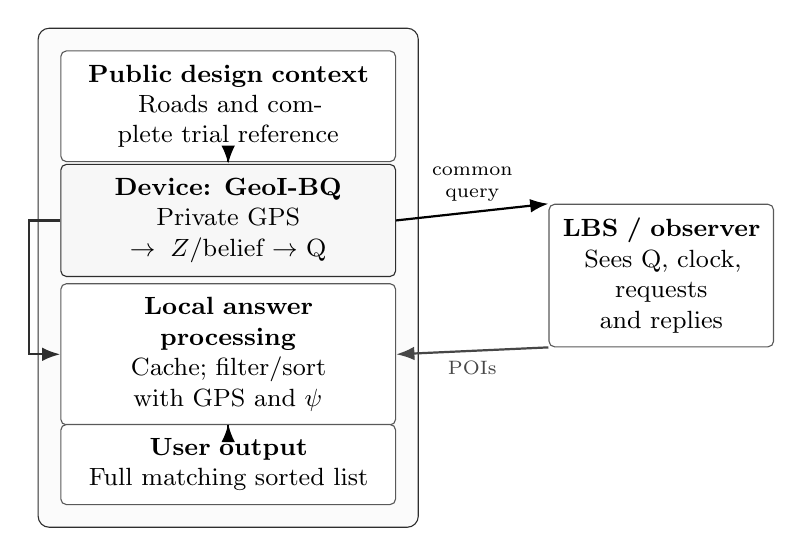
\begin{tikzpicture}[>=Latex,
 box/.style={draw=ink!65,rounded corners=2pt,fill=white,text width=3.9cm,
 align=center,inner sep=5pt,font=\small},
 arr/.style={->,thick,draw=ink}]
\node[box,draw=teal,fill=teal!4] (model) at (0,0)
{\textbf{Device: GeoI-BQ}\\Private GPS $\to Z$/belief $\to$ Q};
\node[box] (local) at (0,-1.7)
{\textbf{Local answer processing}\\Cache; filter/sort with GPS and $\psi$};
\node[box,text width=2.5cm] (server) at (5.5,-.7)
{\textbf{LBS / observer}\\Sees Q, clock,\\requests and replies};
\node[box,text width=3.9cm] (context) at (0,1.45)
{\textbf{Public design context}\\Roads and complete trial reference};
\node[box] (out) at (0,-3.1)
{\textbf{User output}\\Full matching sorted list};
\draw[arr] (context)--(model);
\draw[arr] (model.east)--node[above,font=\scriptsize,align=center]{common\\query}(server.north west);
\draw[arr,blue] (server.south west)--node[below,font=\scriptsize]{POIs}(local.east);
\draw[arr] (local)--(out);
\draw[arr,teal] (model.west)--++(-.4,0)|-(local.west);
\begin{scope}[on background layer]
\node[fit=(model)(local)(context)(out),draw=teal,fill=teal!2,rounded corners,inner sep=8pt] {};
\end{scope}
\end{tikzpicture}
}
\caption{Trusted device and provider boundary. The prototype already loads the
complete static reference used by the trial provider.}\label{fig:system}
\end{figure}

The guarantees require common candidate support and positive public base masses
at each augmented action prefix, including fake lane states; ideal spatial
kernels; fresh independent uniform Q bits; committed, nonrollbackable session
state and full upstream restoration; public boundaries/clock; and the same
conditional provider law at the same query/history. Movement is exogenous.
Account/IP identifiers, private start/stop timing and feedback require additional
channels. Cache results require valid metadata and a common ranking order.
Integer Q arithmetic alone does not certify the complete floating-point
implementation~\cite{mironov}.

The operational factory has complete reference/reply data matching the static
provider. Received-candidate masks constrain the measured answer, but do not
establish information isolation: an equally informed offline client can answer
all defined static requests exactly. Acquisition and refresh costs remain separate.

\subsection{Protected reference and belief}
The road exponential mechanism (REM) directly samples a road state:
\begin{equation}
R_u(v\mid x)=
\frac{e^{-u\|x-a_v\|/2}}{\sum_{w\in V}e^{-u\|x-a_w\|/2}},
\quad Z=a_v. \label{eq:rem}
\end{equation}
At a permitted later GPS read, the old reference $h$ is tested by
\begin{equation}
D_t=\mathbf1\{\|x_t-h\|+\xi_t>\theta\},
\quad \xi_t\sim\operatorname{Lap}(0,1/u). \label{eq:test}
\end{equation}
Reuse costs $u$; test-and-refresh costs $2u$; the initial REM costs $u$.
A prospective filter reserves the maximal next cost before reading GPS:
\begin{equation}
u\sum_i c_i\le Mu\le C_s,\qquad
M=\lfloor C_s/u\rfloor,\quad c_i\in\{0,1,2\}. \label{eq:cap}
\end{equation}
The frozen configuration uses $u=B/(2H_{\rm cfg})$,
$B=0.24\,\mathrm m^{-1}$ and $H_{\rm cfg}=12$, giving $u=0.01\,\mathrm m^{-1}$,
$M=23$, $C_s=0.23\,\mathrm m^{-1}$ and $\theta=200$ m.
Generally, $C_s\le\log(R_\star)/d_\star$ suffices for spatial ratio $R_\star$
within $D_\infty\le d_\star$. Exhaustion stops new protected reads, not queries.

A representative-state belief predicts using a public motion model and updates
only on an actual protected observation:
\begin{align}
b_t^-(s)&=\sum_r b_{t-1}(r)T_{\Delta t}(r,s),\\
b_t(s)&\propto b_t^-(s)\ell_t(Z_t\mid s,h). \label{eq:belief}
\end{align}
The emission combines the reuse atom with refresh REM likelihood.
A skipped read uses prediction only; repeated Z is not an independent
measurement. This approximate belief is not certified real-user calibration.

\subsection{Bounded segment selection and local answers}
Each action has three K5 frames linked by feasible directed-road movement.
Public context and prior fake actions/replies determine the library and masses;
GPS, Z, belief and request do not prune support. Holding supplies common
feasibility; an empty public construction is a reported failure.
The frozen public planner uses width 24, novelty/long-range weights four and
a 60 s travel scale. The supplement specifies these masses and the bounded
cache-coverage/proximity proxy $g_a(s)$.

Scores $v_a=\sum_sb(s)g_a(s)$ are normalized/quantized to $z_a\in[0,1]$
at resolution 65536. For segment $j$,
\begin{align}
\varepsilon_{Q,j}&=\frac{\Gamma_Q}{j(j+1)},&
\alpha_j&=\frac{\widehat\varepsilon_{Q,j}}{2+\widehat\varepsilon_{Q,j}},\\
\mu_j&=\sum_aw_az_a,&
p_a&=w_a[1+\alpha_j(z_a-\mu_j)]. \label{eq:kernel}
\end{align}
Here $\widehat\varepsilon_{Q,j}\le\varepsilon_{Q,j}$ is the downward-rounded
rational allowance; $\Gamma_Q=1$ in the trial.
Exact integer cumulative weights implement this PMF conditional on uniform bits.

One committed segment emits at offsets 0, 20 and 40 s; the next starts at 60 s
(Fig.~\ref{fig:model}). Protected GPS reads are at least 60 s apart, while
current local GPS can rank at every tick. Each Q requests the same six categories,
$L60$ per category. The device deduplicates/caches replies, then filters and
sorts privately using $\psi_t$. Users receive the full matching list;
top five is only the evaluation reference.

\begin{figure*}[t]\centering
\resizebox{.94\textwidth}{!}{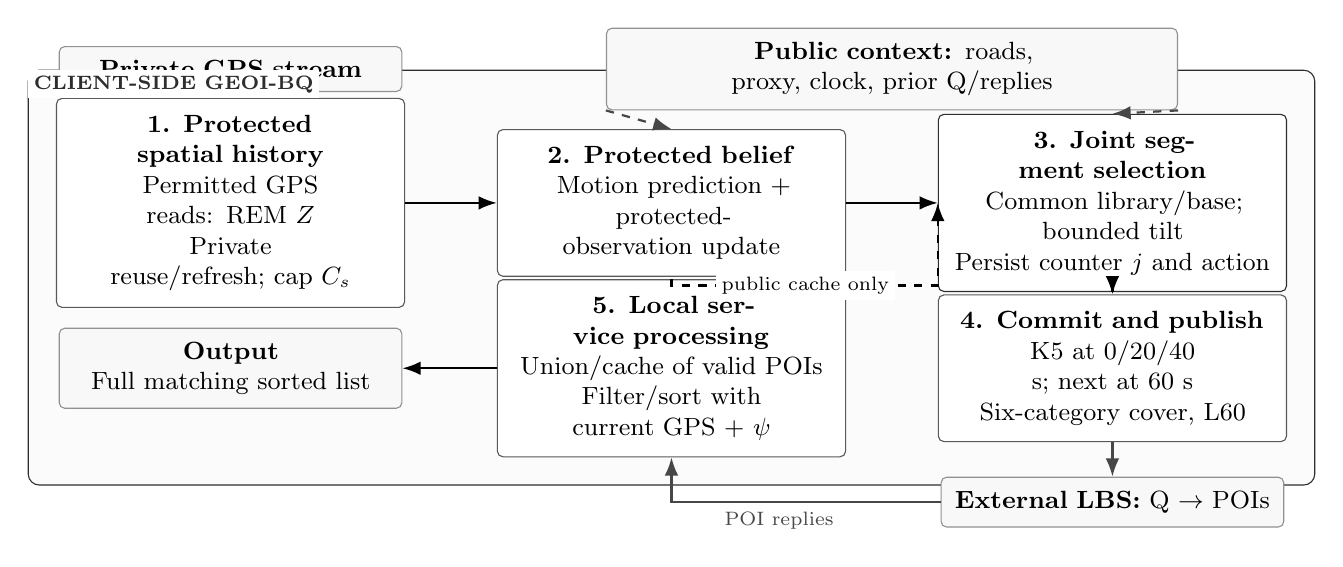
\begin{tikzpicture}[>=Latex,
 box/.style={draw=ink!65,rounded corners=2pt,fill=white,text width=4cm,
 align=center,inner sep=6pt,font=\small},
 side/.style={draw=blue!60,fill=blue!4,rounded corners=2pt,text width=4cm,
 align=center,inner sep=5pt,font=\small},
 arr/.style={->,thick,draw=ink}]
\node[box] (rem) at (0,0)
{\textbf{1. Protected spatial history}\\Permitted GPS reads: REM $Z$\\Private reuse/refresh; cap $C_s$};
\node[box] (belief) at (5.6,0)
{\textbf{2. Protected belief}\\Motion prediction +\\protected-observation update};
\node[box,draw=teal] (choose) at (11.2,0)
{\textbf{3. Joint segment selection}\\Common library/base; bounded tilt\\Persist counter $j$ and action};
\node[box] (send) at (11.2,-2.1)
{\textbf{4. Commit and publish}\\K5 at 0/20/40 s; next at 60 s\\Six-category cover, L60};
\node[box] (local) at (5.6,-2.1)
{\textbf{5. Local service processing}\\Union/cache of valid POIs\\Filter/sort with current GPS + $\psi$};
\node[side] (input) at (0,1.7)
{\textbf{Private GPS stream}};
\node[side,text width=6.9cm] (public) at (8.4,1.7)
{\textbf{Public context:} roads, proxy, clock, prior Q/replies};
\node[side] (output) at (0,-2.1)
{\textbf{Output}\\Full matching sorted list};
\node[side] (provider) at (11.2,-3.8)
{\textbf{External LBS:} Q $\to$ POIs};
\draw[arr] (input)--(rem);
\draw[arr] (rem)--(belief);
\draw[arr] (belief)--(choose);
\draw[arr] (choose)--(send);
\draw[arr] (local)--(output);
\draw[arr,blue] (send)--(provider);
\draw[arr,blue] (provider.west)-|node[below,pos=.3,font=\scriptsize]{POI replies}(local.south);
\draw[arr,dashed,blue] (public.south west)--(belief.north);
\draw[arr,dashed,blue] (public.south east)--(choose.north);
\draw[arr,dashed] (local.north)--(5.6,-1.05)-|(choose.west);
\node[font=\scriptsize,fill=white,inner sep=2pt] at (7.3,-1.05) {public cache only};
\begin{scope}[on background layer]
\node[fit=(rem)(belief)(choose)(send)(local),draw=teal,fill=teal!2,
 rounded corners,inner sep=10pt] (boundary) {};
\end{scope}
\node[font=\scriptsize\bfseries,text=teal,anchor=north west,fill=white,inner sep=2pt]
at (boundary.north west) {CLIENT-SIDE GEOI-BQ};
\end{tikzpicture}
}
\caption{GeoI-BQ workflow. Private spatial history scores a common public
segment library; committed frames retrieve POIs for local ranking.
Only public cache information feeds back into candidate construction.}\label{fig:model}
\end{figure*}

Figure~\ref{fig:walkthrough} traces a retained TEST trip selected for its
multi-turn geometry. At 20/40 s belief predicts without a protected GPS read;
the test-and-refresh steps at 60/120/180 s each spend two units.

\begin{figure*}[t]\centering
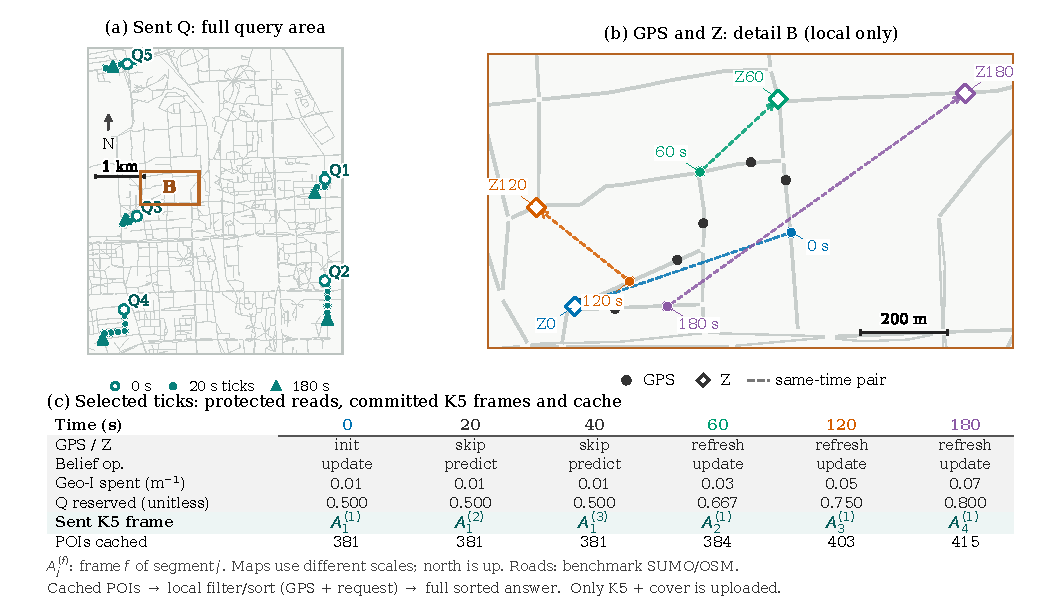
\includegraphics[width=\textwidth]{figure_walkthrough.pdf}
\caption{Retained trip \texttt{cache-046\_day7}, 0--180 s.
(a) All five Q streams; box B locates the separate detail in (b).
Filled GPS and hollow Z markers share time labels/colors; dashed links
show reference displacement, not travel.
(c) Selected ticks and committed frames; the first three share one segment.
Z, belief, ledgers and ranked answers remain local.}\label{fig:walkthrough}
\end{figure*}

\subsection{Privacy analysis}\label{sec:privacy}
Let $X=(x_i)_i$ cover all potential protected-read times, including skipped
ones, and $D_\infty(X,X')=\sup_i\|x_i-x_i'\|$.
The following four statements connect local kernels to the complete wire.
Full proofs and implementation conditions are in the supplement.

\begin{proposition}[Common-domain REM]\label{prop:rem}
Equation~(\ref{eq:rem}) is $u$-Geo-I.
\end{proposition}
\noindent\emph{Proof sketch.}
The reverse triangle inequality bounds both the unnormalized-weight ratio and
the inverse-normalizer ratio by $e^{u\|x-x'\|/2}$.
Multiplication, then summation over outputs/coordinate aliases, gives the event bound.

\begin{proposition}[Private reuse and cap]\label{prop:history}
The ideal protected history $E$ satisfies
\begin{equation}
\Pr_X(E\in B)\le e^{C_sD_\infty(X,X')}\Pr_{X'}(E\in B). \label{eq:history}
\end{equation}
\end{proposition}
\noindent\emph{Proof sketch.}
Distance to fixed $h$ is 1-Lipschitz, so either Laplace threshold event
costs $u$; refresh plus REM costs $2u$.
At every common extended path, chain rule and the prospective ledger bound
the log ratio by $u\sum_i c_i\|x_i-x_i'\|\le C_sD_\infty$.
Marginalizing flags gives (\ref{eq:history}), without independent GPS steps.

\begin{proposition}[Bounded segment kernel]\label{prop:kernel}
For common positive $w$, (\ref{eq:kernel}) is a positive PMF with
$p_a(b)/p_a(b')\le1+\varepsilon_{Q,j}$ for any two beliefs.
\end{proposition}
\noindent\emph{Proof sketch.}
Centering normalizes the PMF and gives
$w_a(1-\alpha_j)\le p_a\le w_a(1+\alpha_j)$.
Their ratio is $1+\widehat\varepsilon_{Q,j}\le1+\varepsilon_{Q,j}$.
Conditional mixtures retain the same bounds.

\begin{proposition}[Adaptive publication]\label{prop:segments}
The complete ordered transcript $O_n$ satisfies
\begin{equation}
\Pr_X(O_n\in B)\le R_n\Pr_{X'}(O_n\in B),\quad
R_n=\prod_{j\le n}(1+\varepsilon_{Q,j})\le e^{\Gamma_Q}. \label{eq:segments}
\end{equation}
\end{proposition}
\noindent\emph{Proof sketch.}
Condition on common augmented prefixes and multiply action bounds.
Committed frames, common-law responses and fixed retries add no ratio factor.
The schedule sums to $\Gamma_Qn/(n+1)$; independent segments are unnecessary.

\begin{theorem}[Conditional end-to-end bound]\label{thm:endtoend}
Under both spatial and publication assumptions,
\begin{equation}
\Pr_X(O_n\in B)\le
e^{\min\{C_sD_\infty(X,X'),\,\log R_n\}}\Pr_{X'}(O_n\in B). \label{eq:endtoend}
\end{equation}
\end{theorem}
\noindent
Post-processing gives the spatial bound; Proposition~\ref{prop:segments}
independently bounds the same event, so their minimum applies.
For $\Gamma_Q=1$, an exact prefix/tail certificate gives
$R_\infty<2.437372$, without a duration limit.
This Q guard can hold without ideal upstream Geo-I; the spatial branch needs
its additional assumptions. With $C_s=0.23\,\mathrm m^{-1}$, the coarse spatial
and Q ceilings cross at approximately 3.874 m.

A uniform ratio $R$ limits posterior event probability to
$f_R(\pi)=R\pi/[1+(R-1)\pi]$ at prior $\pi$.
For radius $r$, put
$\pi_{\max,t}(r)=\sup_y\Pr(\|X_t-y\|\le r\mid C)$.
Every measurable estimator obeys
\begin{equation}
\Pr(\|X_t-\widehat x_t(O)\|\le r\mid C)
\le f_R(\pi_{\max,t}(r)). \label{eq:hit}
\end{equation}
Apply the event bound to the output-selected ball, then average.
Balanced binary priors give posterior below 70.91\% for one session;
strong priors can make this uninformative. Conditional joint-channel ratios
multiply, even for correlated inputs: two valid sessions permit a ceiling
below 85.5925\%. Marginal per-user bounds alone do not establish this premise;
a Raw partner can reveal correlated targets directly.

\subsection{Utility analysis and scope}\label{sec:utility}
At fixed local history, with actual action rewards $r_a\in[0,1]$,
\begin{align}
\E_pz-\E_wz&=\alpha\Var_w(z)\ge0,\\
\E_pr-\E_wr&=\alpha\Cov_w(z,r). \label{eq:gain}
\end{align}
Thus score improvement does not imply actual Recall gain.
A proxy error $|r_a-v_a|\le\eta$ gives lower gain
$\alpha[\Cov_w(z,v)-\eta\E_w|z-\E_wz|]$; unknown error is not zero.

For full-catalogue reference top-$k$ $T_t\ne\varnothing$ and valid received
set $U_t$, common filtering/order gives
\begin{equation}
\operatorname{Recall@}k=\frac{|T_t\cap U_t|}{|T_t|}. \label{eq:recall}
\end{equation}
Cache inclusion cannot reduce Recall at the same GPS/request, but cannot
create absent metadata or ensure monotonicity while the user moves.

Let $P_n$ be the adaptive wire law and $W_n$ the identical policy with
$\Gamma_Q=0$, holding other conditions fixed. Conditional second moments give
\begin{equation}
|\E_{P_n}h-\E_{W_n}h|
\le\frac12\sqrt{\prod_{j\le n}(1+\alpha_j^2/4)-1},
\quad 0\le h\le1. \label{eq:tv}
\end{equation}
The uniform ceiling is below 0.0553 for $\Gamma_Q=1$.
Latent scores are replaced by conditional mean scores, still in $[0,1]$.
This bounds deviation from a matched base, not absolute quality.

If a history-conditional public case law gives proxy reward at least $c$,
actual-case TV error is at most $\tau$, and mean proxy error is at most $\nu$,
then actual expected reward is at least $\max(0,c-\tau-\nu)$.
Conditional expectation extends this to public-weighted session averages without
IID steps. Real calibration remains uncertified.
Finally, purpose-independent payloads provide fixed-context request
noninterference, not secrecy of intent correlated with movement.

\section{Experiments and Analysis}\label{sec:evaluation}
\subsection{Environment Settings}
\subsubsection{Data and evaluation protocol.}
Suppose one method sends a coordinate and another inserts two extra fake
packets. An observer given the same number of packets may see different
portions of the trip. We therefore run each method on the same trips and
score it over the same time windows. GPS at each tick supplies the reference
for localization. The POIs that satisfy the request at that position supply
the reference for service quality. To obtain both, we generate paired route
alternatives in SUMO on a common road map and match them to a POI catalogue.
Public geometry determines trip eligibility before any defense is scored.
Related trips stay together when we split route families.

Native SUMO mobility~\cite{sumo} uses a versioned directed network
(66,189 road states, 4,849 external and 21,179 internal edges) and
418 POIs in six categories with OpenStreetMap provenance~\cite{osm}.
The 48 route families split into 20 TRAIN, 8 SELECTION and 20 TEST.
Two retained trips/family and three TEST draws yield 120 test trip-draws/arm.
Each window lasts 600 s with 31 service ticks. This inspected synthetic cohort
is a controlled comparison, not untouched-city confirmation.

All arms share the catalogue, L60/category/coordinate and local ranking.
Four purposes cover nearest road distance, fastest travel, within 1,000 m,
and minimum detour to a private local destination.
Session cache is primary; empty references are N/A.
Hit100 and Euclidean MAE measure localization; Recall@5 measures answers.
Results aggregate within trip, family, then across families.
We report 10,000 family-bootstrap 95\% intervals~\cite{efron};
repeated draws are not independent families.

\subsubsection{Comparison methods and attackers.}
We compare Raw GPS, direct REM-Z (K1), three starred paper adaptations and
frozen GeoI-BQ v1. TransProtect* uses a Markov predictor (K10,
$\alpha_{\rm TP}=10000$, $\varepsilon=0.005\,\mathrm m^{-1}$);
Semantic* uses OSM/empirical K5 dummies; Fake queries* uses K5
road/history sets with up to two inserted events at 5--15 s waits.
Their differing guarantees, costs and outputs are retained, without equal-epsilon
or official-reproduction claims. Full settings appear in the supplement.

The bank includes geometry/history estimators, ExtraTrees
(64 trees)~\cite{extratrees}, shadow kNN-1/kNN-5 and priors.
Fit uses TRAIN; robust SELECTION is loss-specific; TEST features contain
only public wire, excluding Z, true-member labels and evaluator indices.
S1 sees one packet; S2 sees 540--600 s and targets mean final-window GPS
(a coordinate proxy); S3 reconstructs all ticks from the whole wire;
S9/S10 infer endpoints from the same whole window with public boundaries.
All fake events count. Hit and MAE can select different attackers.

\subsection{Empirical Experiments}
\subsubsection{Main results.}
\begin{table*}[t]\centering\footnotesize
\caption{Localization results: Hit100 (\%, lower) / MAE (m, higher). Same time windows.}\label{tab:privacy}
\begin{tabularx}{\linewidth}{@{}P{2.7cm}CCCCC@{}}\toprule
\textbf{Method} & \textbf{S1} & \textbf{S2} & \textbf{S3} & \textbf{S9} & \textbf{S10} \\
\midrule
Raw GPS & 100.000 / 0.0 & 100.000 / 0.0 & 100.000 / 0.0 & 100.000 / 0.0 & 100.000 / 0.0 \\
REM-Z (K1) & 18.522 / 338.5 & 37.500 / 214.3 & 18.522 / 338.5 & 5.833 / 435.8 & 35.000 / 246.8 \\
TransProtect* & 82.984 / 54.4 & 94.167 / 28.7 & 82.984 / 54.4 & 96.667 / 17.8 & 90.833 / 33.6 \\
Semantic* & 82.258 / 41.9 & 100.000 / 8.2 & 82.258 / 41.9 & 100.000 / 5.3 & 100.000 / 7.3 \\
Fake queries* & 53.387 / 1213.0 & 92.500 / 239.1 & 98.790 / 13.3 & 99.167 / 42.2 & 100.000 / 6.4 \\
\textbf{GeoI-BQ v1} & 0.188 / 2104.6 & 0.000 / 2124.2 & 0.188 / 2104.6 & 0.000 / 1986.4 & 0.000 / 2124.2 \\
\bottomrule\end{tabularx}
\par\smallskip\raggedright * Audited adaptations, not official author implementations. Each loss has its own selected attacker. Full CIs appear in the supplement.
\end{table*}

\begin{table*}[t]\centering\footnotesize
\caption{Session Recall@5 (\%, higher) by purpose and acquisition cost per 600 s.}\label{tab:service}
\begin{tabularx}{\linewidth}{@{}P{2.7cm}CCCCCCC@{}}\toprule
\textbf{Method} & \textbf{Macro} & \textbf{Nearest} & \textbf{Fastest} & \textbf{Radius} & \textbf{Detour} & \textbf{Coordinates} & \textbf{Reply KB} \\
\midrule
Raw GPS & 99.999 & 100.000 & 100.000 & 100.000 & 99.995 & 31.00 & 16.843 \\
REM-Z (K1) & 99.700 & 99.753 & 99.753 & 99.625 & 99.668 & 31.00 & 16.921 \\
TransProtect* & 99.996 & 100.000 & 100.000 & 100.000 & 99.986 & 31.00 & 16.847 \\
Semantic* & 99.999 & 100.000 & 100.000 & 100.000 & 99.997 & 155.00 & 84.770 \\
Fake queries* & 99.999 & 100.000 & 100.000 & 100.000 & 99.997 & 190.21 & 104.033 \\
\textbf{GeoI-BQ v1} & 99.595 & 99.638 & 99.641 & 99.388 & 99.712 & 155.00 & 82.557 \\
\bottomrule\end{tabularx}
\par\smallskip\raggedright KB = 1,000 bytes of reply-index JSON; full records, transport overhead, latency and energy are excluded.
\end{table*}

Raw recovers observed coordinates exactly; all six arms complete 120/120 draws
without failures. GeoI-BQ yields Hit100 0--0.188\% and MAE 1.99--2.12 km,
versus REM-Z Hit100 5.833--37.500\%.
Fake queries* illustrates the value of temporal evaluation: S1 has
53.387\% Hit100 / 1,213 m MAE, but S3 has 98.790\% / 13.3 m.
The known clock and history undermine this adaptation's inserted events.
These are retained-bank results, not universal rankings or Bayes-optimal attacks;
zero-hit intervals do not prove zero population risk.

GeoI-BQ's macro Recall is 99.595\%, CI [99.224, 99.903]\%.
Against TransProtect*, the paired difference is $-0.401$ pp,
CI [$-0.773$,$-0.093$]; utility superiority is not supported.
It uses 155 coordinate queries versus 31 for singleton arms and approximately
190.21 for Fake queries*. Byte counts serialize reply indices rather than full
records; replayed REM-Z/GeoI-BQ generation latency is unavailable.
Source-metric comparison is partial. Singleton travel-cost distortion from
TransProtect's Eq.~13 gives 47.44 m for TransProtect* and 688.65 m for REM-Z
using eight local TRAIN-selected targets/prior. This is a local proxy, not the
original cities or VehiTrack reproduction. Q-only output has no unique
singleton for that metric. Source-calibrated ASR, DER and path counts remain
N/A where inputs or contracts are incompatible; reasons and full CIs are retained
in the supplement.

\subsubsection{Extended tasks and attribution.}
S4 route-family association gives GeoI-BQ balanced accuracy 47.50\%,
CI [40.00, 54.17]\%, without physical person/vehicle labels.
S5 is inconclusive because Raw is also at 50\%.
S6 post-turn destination choice is informative: Raw reaches 100\%,
adaptations 95--99.17\%, GeoI-BQ 50.83\%
(CI [44.17, 57.50]\%); REM-Z is also at chance.
S7's common wrapper yields identical wire across 1,056 streams and 25,344
purpose/category counterfactuals. This fixed-context property is shared,
not unique to GeoI-BQ or evidence against correlated-intent inference.
Post-V1 S8 fusion raises Semantic*/Fake-query* protected-partner Hit100 to
75\%/68.33\%, while GeoI-BQ has no retained hits.
An available perfectly aligned Raw-partner estimator reaches 100\% in every arm.
These extensions are diagnostics on the inspected cohort.

High Recall partly reflects catalogue saturation: the first GeoI-BQ packet
acquires 380.2/418 unique POIs on average, and the final cache 415.875.
Current/epoch/session Recall is 96.780/97.123/99.595\%.
The matched $\Gamma_Q=0$ base achieves 99.711\%; proposed minus base is
$-0.116$ pp, CI [$-0.253$,$-0.006$]. Private adaptation is therefore not
shown necessary for quality. Complete client reference access also permits exact
offline static answers under equal information, without implying zero setup cost.

All ledgers spend 13--21 of 23 units: the 600 s trial never exhausts its cap.
Long-trip utility, unknown/dynamic provider data, new geography, practical entropy,
upstream numerical/restoration guarantees and additional identity channels remain
outside the demonstrated result.

\section{Summary}\label{sec:conclusion}
GeoI-BQ separates protected spatial history from bounded query publication.
Under stated conditions, four local-to-session results yield a complete
transcript bound and prior-dependent inference consequences. Utility analysis
distinguishes exact cache/ranking properties, planning-score gain and conditional
service guarantees.

The controlled comparison combines low localization Hit100 with 99.595\%
session Recall at higher query cost. However, the public base performs slightly
better, complete-reference access weakens online-necessity claims, and post-cap
utility is untested. The contribution is an auditable conditional mechanism and
comparison, with deployment certification, faithful source-paper reproduction
and independent mobility/provider evaluation remaining future work.

\begin{credits}
\subsubsection{Data and code availability.}
Synthetic mobility, geographic snapshots, code and frozen artifact hashes are indexed
by the accompanying manifest. Original geographic licenses apply.
A persistent publication archive remains to be registered.
\subsubsection{Declaration of generative AI assistance.}
OpenAI ChatGPT/Codex assisted drafting, software preparation and consistency checks.
The authors remain responsible for final verification, editing and approval.
\end{credits}
\bibliographystyle{splncs04}
\bibliography{references}
\end{document}
